\clearpage{\pagestyle{empty}\cleardoublepage}

\chapter{\htx\ analysis: comparison of signal prediction between singlet and doublet scenarios}
%\section{Comparison of signal prediction between singlet and doublet scenarios}
\label{app:SingletvsDoublet}

As discussed in Sect.~\ref{sec:SimulatedSamples}, the signal MC samples used in this analysis were
generated in the singlet scenario, for which the mixing between the $\T$ quark and SM quarks is left-handed.
For simplicity, these samples are reweighted to reproduce any desired branching-ratio configuration, included
that corresponding to a doublet scenario. There is a small concern that for the latter the mixing between the $\T$
quark and SM quarks is right-handed, slightly affecting the kinematics and thus the signal acceptance and shape
of the $\HT$ distribution. Two MC samples for the doublet scenario, corresponding to $m_{\T}=350$ and $600\gev$, are available, which
have been used to check this effect. Figure~\ref{fig:HT_checks_SingletvsDoubletComp} compares, for both mass
points and each of the three analysis channels considered, the yield and shape of the $\HT$ distribution for the 
predicted signal using the singlet and doublet samples. In both cases the samples were reweighted to reproduce
the branching ratios corresponding to the doublet model. As it can be appreciated, the shapes of the distributions
are in reasonable agreement and discrepancies in the yields are below 5\% in the highest-sensitivity channel ($\geq 4$ $b$ tags).

%%%%%%%%%%%%%%
\begin{figure}[htbp]
\begin{center}
\subfigure[]{\label{fig:singletdoublet_2b}
\includegraphics[width=0.32\textwidth]{htx_analysis_14ifb/figures/doubletcomp_HTAll_ELEMUON_6jetin2btagex_NOMINAL.eps}}
\subfigure[]{\label{fig:singletdoublet_3b}
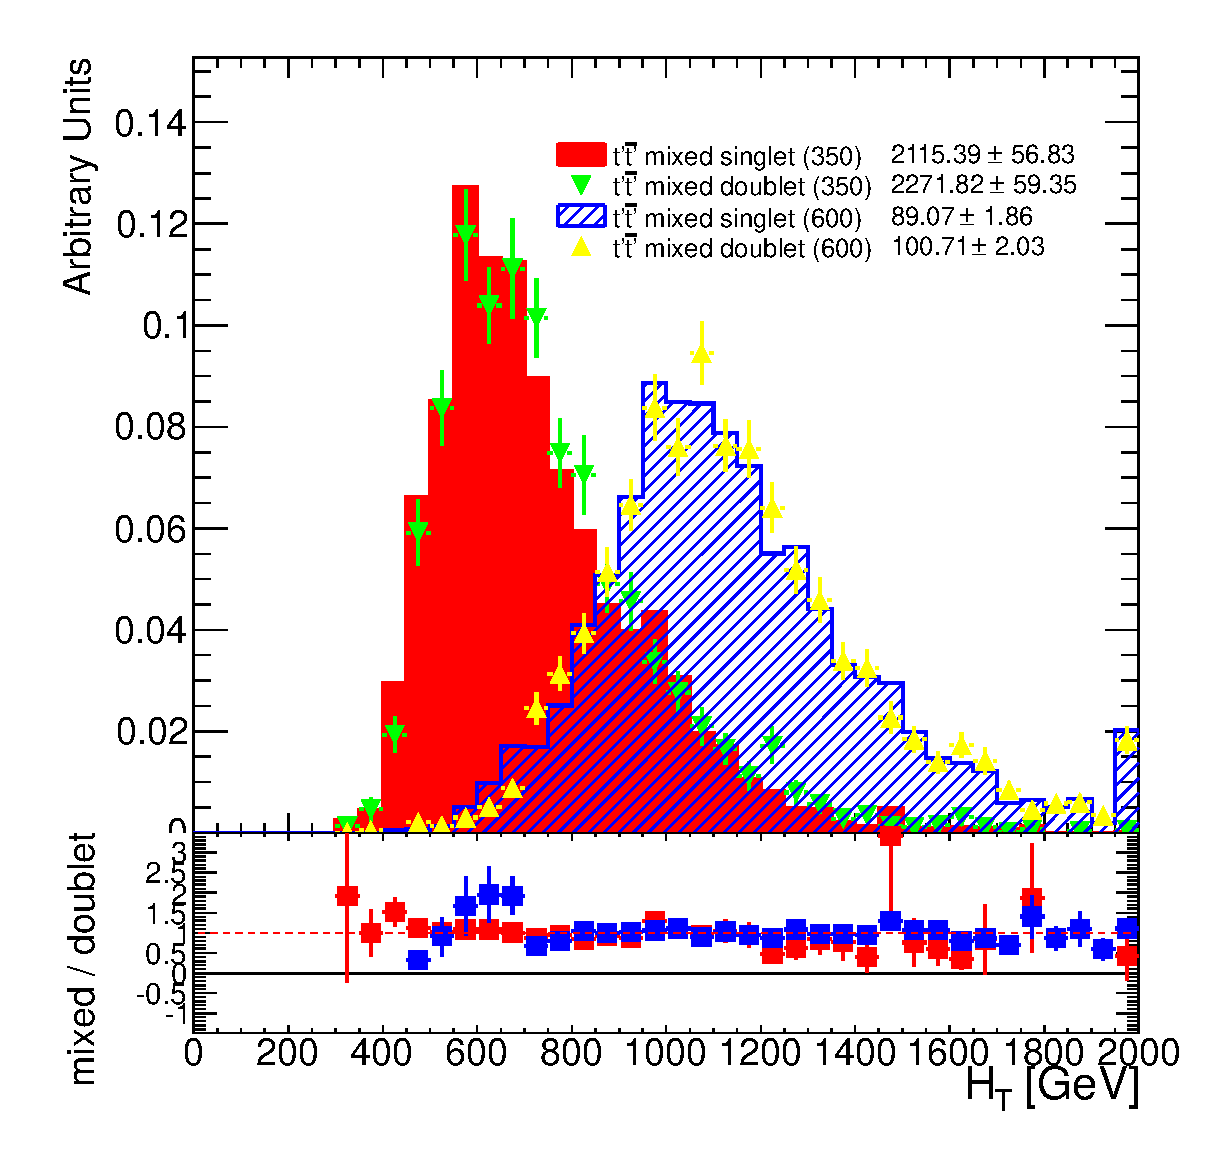
\includegraphics[width=0.32\textwidth]{htx_analysis_14ifb/figures/doubletcomp_HTAll_ELEMUON_6jetin3btagex_NOMINAL.eps}}
\subfigure[]{\label{fig:singletdoublet_4b}
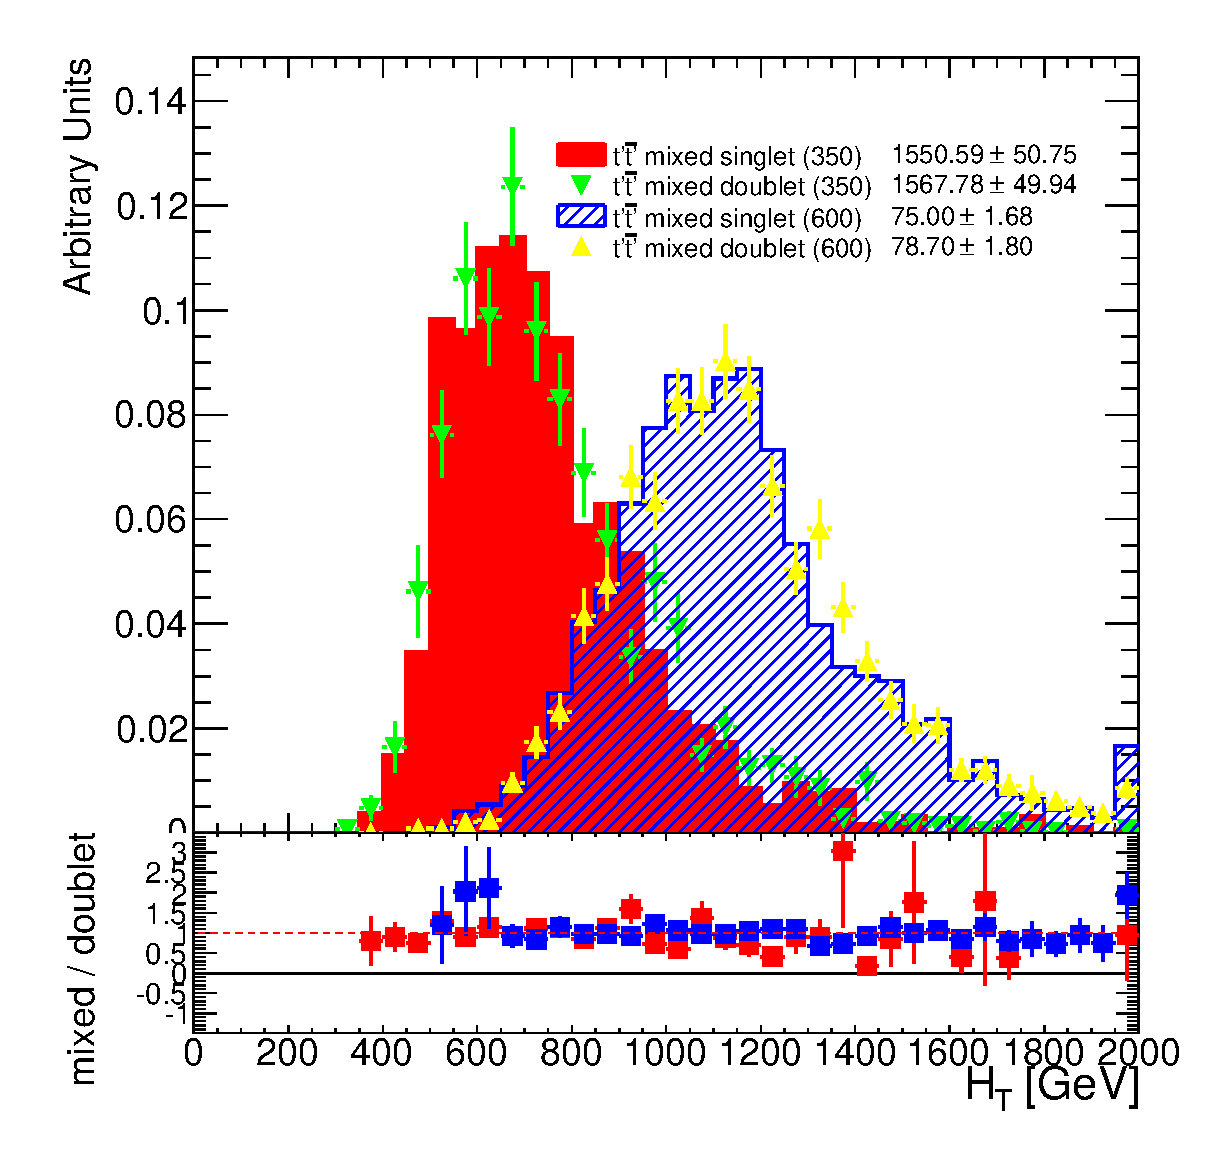
\includegraphics[width=0.32\textwidth]{htx_analysis_14ifb/figures/doubletcomp_HTAll_ELEMUON_6jetin4btagin_NOMINAL.eps}}
\caption{
Comparison of the yields and shape of the $\HT$ distribution in simulation for $\T$ signal using the singlet samples (symbols) and
using the doublet samples (histogram). In both cases the signal has been reweighted to reproduce the branching ratios corresponding 
to the doublet model. The selection used corresponds to the combined $e$+jets and $\mu$+jets channels
with $\geq 6$ jets and (a) 2 $b$ tags,  (b) 3 $b$-tags and (c) $\geq 4$ $b$ tags. The comparison is made for two 
different mass points, $m_{\T}=350$ and $600\gev$.
The last bin in all figures contains the overflow.
\label{fig:HT_checks_SingletvsDoubletComp}}
\end{center}
\end{figure}
%%%%%%%%%%%%%%
